\documentclass[tikz,border=8pt]{standalone}

\usetikzlibrary{arrows.meta,positioning,fit,backgrounds}

\definecolor{synblue}{HTML}{2B6CB0}
\definecolor{syngreen}{HTML}{2F855A}
\definecolor{synorange}{HTML}{DD6B20}
\definecolor{synred}{HTML}{C53030}
\definecolor{synpurple}{HTML}{6B46C1}
\definecolor{textgray}{HTML}{2D3748}

\begin{document}

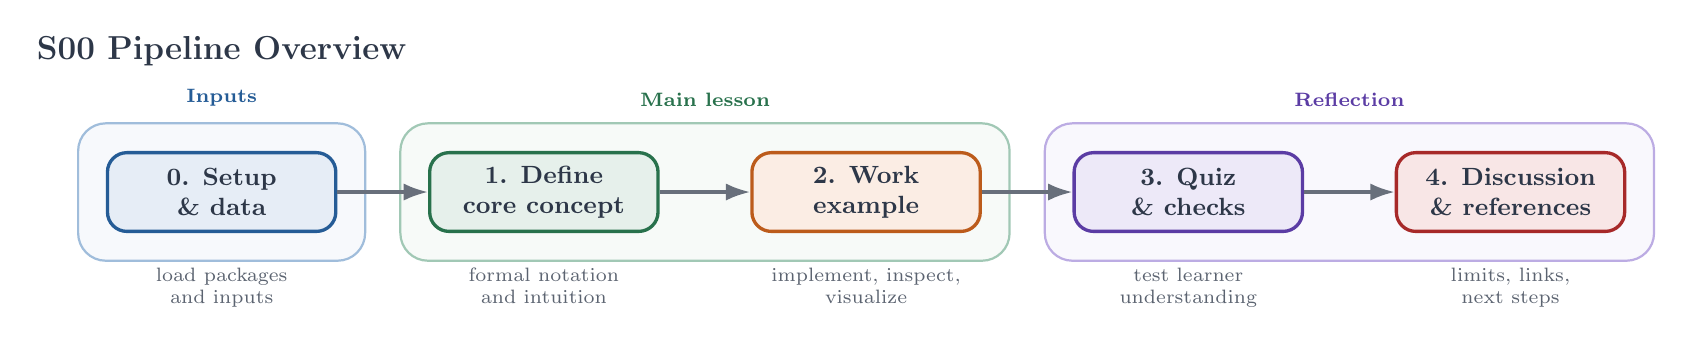
\begin{tikzpicture}[
    font=\sffamily,
    every node/.style={text=textgray},
    title/.style={
        font=\large\bfseries,
        text=textgray
    },
    step/.style={
        rectangle,
        rounded corners=7pt,
        minimum width=2.9cm,
        minimum height=1.0cm,
        align=center,
        font=\small\bfseries,
        very thick,
        draw=#1!85!black,
        fill=#1!12
    },
    note/.style={
        font=\scriptsize,
        align=center,
        text=textgray!78
    },
    arrow/.style={
        -{Latex[length=3.1mm,width=2.2mm]},
        very thick,
        draw=textgray!72
    },
    phase/.style={
        rectangle,
        rounded corners=10pt,
        draw=#1!45,
        fill=#1!4,
        thick,
        inner xsep=10pt,
        inner ysep=10pt
    },
    phaselabel/.style={
        font=\scriptsize\bfseries,
        text=#1!85!black
    }
]

\node[title] (title) {S00 Pipeline Overview};

\node[step=synblue, below=0.95cm of title] (setup)
{0. Setup\\\& data};

\node[step=syngreen, right=1.15cm of setup] (concept)
{1. Define\\core concept};

\node[step=synorange, right=1.15cm of concept] (example)
{2. Work\\example};

\node[step=synpurple, right=1.15cm of example] (practice)
{3. Quiz\\\& checks};

\node[step=synred, right=1.15cm of practice] (discussion)
{4. Discussion\\\& references};

\draw[arrow] (setup) -- (concept);
\draw[arrow] (concept) -- (example);
\draw[arrow] (example) -- (practice);
\draw[arrow] (practice) -- (discussion);

\node[note, below=0.32cm of setup]
{load packages\\and inputs};
\node[note, below=0.32cm of concept]
{formal notation\\and intuition};
\node[note, below=0.32cm of example]
{implement, inspect,\\visualize};
\node[note, below=0.32cm of practice]
{test learner\\understanding};
\node[note, below=0.32cm of discussion]
{limits, links,\\next steps};

\begin{scope}[on background layer]
    \node[phase=synblue, fit=(setup)] (p0) {};
    \node[phase=syngreen, fit=(concept)(example)] (p1) {};
    \node[phase=synpurple, fit=(practice)(discussion)] (p2) {};
\end{scope}

\node[phaselabel=synblue, above=0.08cm of p0.north] {Inputs};
\node[phaselabel=syngreen, above=0.08cm of p1.north] {Main lesson};
\node[phaselabel=synpurple, above=0.08cm of p2.north] {Reflection};

\end{tikzpicture}

\end{document}
